\documentclass[10pt]{beamer}

\usetheme{metropolis}
\usepackage{appendixnumberbeamer}

\usepackage{booktabs}
\usepackage[scale=2]{ccicons}

\usepackage{pgfplots}
\usepgfplotslibrary{dateplot}

\usepackage{xspace}
\newcommand{\themename}{\textbf{\textsc{metropolis}}\xspace}

\usepackage{ctex,listings}
\title{Project2: User Programs}
\subtitle{PintOS}
\date{\today}
\author{陈震雄}
\institute{武汉大学}
% defs
\def\cmd#1{\texttt{\color{red}\footnotesize $\backslash$#1}}
\def\env#1{\texttt{\color{blue}\footnotesize #1}}

\definecolor{deepblue}{rgb}{0,0,0.5}
\definecolor{deepred}{rgb}{0.6,0,0}
\definecolor{deepgreen}{rgb}{0,0.5,0}
\definecolor{halfgray}{gray}{0.55}

\lstset{
    basicstyle=\ttfamily\tiny,
    keywordstyle=\bfseries\color{deepblue},
    emphstyle=\ttfamily\color{deepred},
    stringstyle=\color{deepgreen},
    numbers=left,
    numberstyle=\tiny\color{halfgray},
    showspaces=false,
    commentstyle=\color{halfgray}
}

\titlegraphic{\hfill
\includegraphics[height=2cm]{figures/whulogo.pdf}}

\logo{
\includegraphics[height=1cm]{figures/whulogo.pdf}}

\begin{document}

\maketitle

\begin{frame}{Table of contents}
  \setbeamertemplate{section in toc}[sections numbered]
  \tableofcontents[hideallsubsections]
\end{frame}

\section{Introduction}
\begin{frame}{Introduction}
    Now that you've worked with Pintos and are becoming familiar with its infrastructure and thread package, \textbf{it's time to start working on the parts of the system that allow running user programs.}

\textbf{The base code already supports loading and running user programs, but no I/O or interactivity is possible.} In this project, you will enable programs to interact with the OS via system calls.

You will be working out of the userprog/ directory for this assignment, but you will also be interacting with almost every other part of Pintos. We will describe the relevant parts below.
\end{frame}
%-------prepare-----------------
\section{Preparation}
\begin{frame}[fragile]{Problem1}
    \begin{figure}
        \centering
    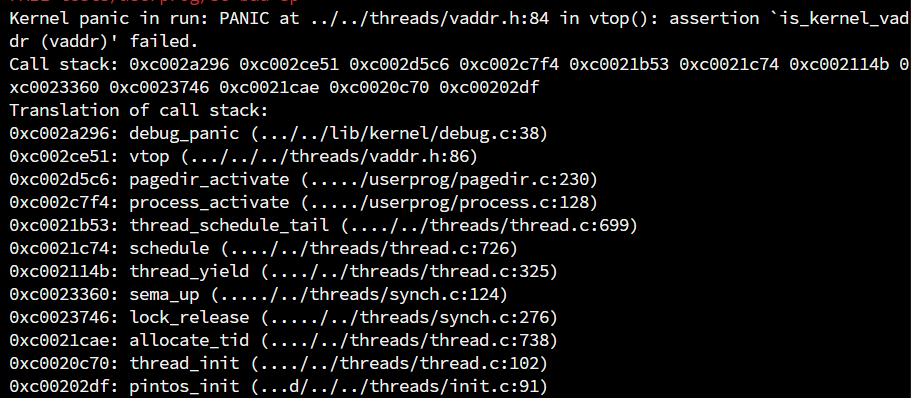
\includegraphics[width=\linewidth]{figures/erro1.png}
    \end{figure}
  paging\_init () is called after thread\_init(). So the assertion is false.
\end{frame}
%---
\begin{frame}[fragile]{Problem2}
    \begin{lstlisting}[language=C]
// thread.c
static bool schedule_started;

void thread_start (void) {
  schedule_started = true;
  ...
}

void thread_yield (void) {
  if (!schedule_started)
    return;
  ...
}
    \end{lstlisting}
\begin{figure}
    \centering
    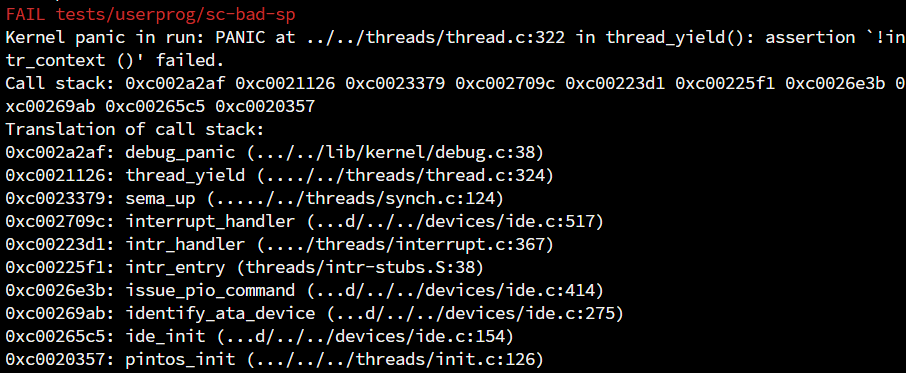
\includegraphics[width=0.8\linewidth]{figures/erro2.png}
\end{figure}
thread\_yied() can't be called in intr\_context().
\end{frame}
%_------
\begin{frame}[fragile]{Problem3}
    \begin{lstlisting}[language=C]
// synch.c
void sema_up (struct semaphore *sema) {
    ...
     if (intr_context ())
        intr_yield_on_return ();
    else
        thread_yield ();
    ...
}
    \end{lstlisting}
    pintos -v -k -T 360 --qemu\\  
    --filesys-size=2 \\
    -p tests/userprog/no-vm/multi-oom\\
    -a multi-oom \\ 
    -- \\
    -q  -f run \textbf{multi-oom} 
\end{frame}

\begin{frame}[fragile]{Push args}
\begin{columns}
\begin{column}{0.5\textwidth}
\begin{lstlisting}[language=C]
// process.c
static void push_arguments (const char* cmdline_tokens[], int argc, void **esp)
{
  ASSERT(argc >= 0);
  int i, len = 0;
  void* argv_addr[argc];
  /* push argvs into **esp */
  for (i = argc - 1; i >= 0; i--) {
    len = strlen(cmdline_tokens[i]) + 1;
    *esp -= len;
    memcpy(*esp, cmdline_tokens[i], len);
    argv_addr[i] = *esp;
  }
  /* word align to 4 bytes. */
  *esp = (void*)((unsigned int)(*esp) & 0xfffffffc);
  /* push null, indicating the end of argv. */
  *esp -= 4;
  *((uint32_t*) *esp) = 0;
  /* push argvs address into **esp. */
  for (i = argc - 1; i >= 0; i--) {
    *esp -= 4;
    *((void**) *esp) = argv_addr[i];
  }
  /* push **argv (addr of stack, esp). */
  *esp -= 4;
  *((void**) *esp) = (*esp + 4);
  /* push argc. */
  *esp -= 4;
  *((int*) *esp) = argc;
  /* push ret addr. */
  *esp -= 4;
  *((int*) *esp) = 0;
}
\end{lstlisting}
\end{column}
\begin{column}{0.5\textwidth}
\begin{lstlisting}[language=C]
static void
start_process(void *pcb_)
{
  ...
  /* Tokenize the command line. */
  char *token;
  char *save_ptr;
  int cnt = 0;
  for (token = strtok_r(file_name, " ", &save_ptr); 
      token != NULL;
      token = strtok_r(NULL, " ", &save_ptr))      
      cmdline_tokens[cnt++] = token;
  /* If load succeeds, push arguments to the stack. */
  if (success) {
    push_arguments(cmdline_tokens, cnt, &if_.esp);
  }
  ...
}
\end{lstlisting}
Now, PintOS can accept user program's args.
\end{column}
\end{columns}
\end{frame}
%----------------------
\section{Task 1: Process Termination Messages}
\begin{frame}{Exercise 1.1}
    Whenever a user process terminates, because it called exit or for any other reason, print the process's name and exit code, formatted as if printed by printf ("\%s: exit(\%d)\textbackslash n", ...);.

The name printed should be the full name passed to process\_execute(), omitting command-line arguments.

Do not print these messages when a kernel thread that is not a user process terminates, or when the halt system call is invoked. The message is optional when a process fails to load.

Aside from this, don't print any other messages that Pintos as provided doesn't already print. You may find extra messages useful during debugging, but they will confuse the grading scripts and thus lower your score.

\textbf{Print exit message} formatted as "\%s: exit(\%d)\textbackslash n" with process name and exit status when process is terminated.
\end{frame}
\begin{frame}[fragile]{Exercise 1.1}
    \begin{lstlisting}[language=C]
// syscall.c
static void
syscall_handler (struct intr_frame *f UNUSED) 
{
    ...
    case SYS_EXIT:
    {
      int exitcode;
      memread_user(f->esp + 4, &exitcode, sizeof(exitcode));
      sys_exit(exitcode);
      NOT_REACHED();
      break;
    }
    ...
}
void 
sys_exit(int status UNUSED) 
{
  printf("%s: exit(%d)\n", thread_current()->name, status);

  thread_exit();
}
    \end{lstlisting}
\end{frame}
%-------
\section{Task 2: Argument Passing}
\begin{frame}[fragile]{Exercise 2.1}
        Currently, process\_execute() does not \textbf{support passing arguments} to new processes. You need to implement it in this task.

Implement this functionality, by extending process\_execute() so that instead of simply taking a program file name as its argument, it divides it into words at spaces.

The first word is the program name, the second word is the first argument, and so on. That is, process\_execute("grep foo bar") should run grep passing two arguments foo and bar.

Within a command line, multiple spaces are equivalent to a single space, so that process\_execute("grep foo bar") is equivalent to our original example.

You can impose a reasonable limit on the length of the command line arguments. For example, you could limit the arguments to those that will fit in a single page (4 kB). (There is an unrelated limit of 128 bytes on command-line arguments that the pintos utility can pass to the kernel.)
\end{frame}
%-------
\section{Task 3: Accessing User Memory}
\begin{frame}{Exercise 3.1}
    As part of a system call, the kernel must often access memory through pointers provided by a user program.

The kernel must be very careful about doing so, because the user can pass a null pointer, a pointer to unmapped virtual memory, or a pointer to kernel virtual address space (above PHYS\_BASE).

All of these types of invalid pointers must be rejected without harm to the kernel or other running processes, by terminating the offending process and freeing its resources.

\textbf{Support reading from and writing to user memory for system calls.}
\textbf{In either case, you need to make sure not to "leak" resources.}
\textbf{An invalid user pointer will cause a "page fault"}
\end{frame}
%---
\begin{frame}[fragile]{Basic mem access funcs.}
\begin{lstlisting}[language=C]
// syscall.c
static int32_t
get_user (const uint8_t *uaddr) 
{
  /* check that a user pointer `uaddr` points below PHYS_BASE*/
  if (! ((void*)uaddr < PHYS_BASE))
    return -1; /**< invalid memory access */

  /* as suggested in the reference manual, see (3.1.5) */
  int result;
  asm ("movl $1f, %0; movzbl %1, %0; 1:"
      : "=&a" (result) : "m" (*uaddr));
  return result;
}
static bool
put_user (uint8_t *udst, uint8_t byte) 
{
  /* check that a user pointer `udst` points below PHYS_BASE */
  if (! ((void*)udst < PHYS_BASE)) 
    {
      return false;
    }
  int error_code;

  /* as suggested in the reference manual, see (3.1.5) */
  asm ("movl $1f, %0; movb %b2, %1; 1:"
      : "=&a" (error_code), "=m" (*udst) : "q" (byte));
  return error_code != -1;
}
\end{lstlisting}
\end{frame}
\begin{frame}[fragile]{More user mem access funcs and page\_fault.}
\begin{columns}
\begin{column}{0.5\textwidth}
\begin{lstlisting}[language=C]
// syscall.c
/** check a single byte is in user mem. */
static void
check_user (const uint8_t *uaddr) 
{
  /* check uaddr range or segfaults */
  if(get_user (uaddr) == -1)
    fail_invalid_access();
}
static bool 
validate_user_string(const char *uaddr) 
{
  const char *p = uaddr;
  size_t max_len = 1024; 
  while (max_len--) {
    int c = get_user((const uint8_t *)p);
    if (c == -1) return false;
    if (c == 0) return true;
    p++;
  }
  return false;
}
\end{lstlisting}
\end{column}
\begin{column}{0.5\textwidth}
\begin{lstlisting}[language=C]
static int 
fail_invalid_access(void) 
{
  if (lock_held_by_current_thread(&filesys_lock))
    lock_release (&filesys_lock);
  sys_exit (-1);
  NOT_REACHED();
}
// exception.c
static void
page_fault (struct intr_frame *f) 
{
    ...
    /* (3.1.5) a page fault in the kernel merely 
    sets eax to 0xffffffff and copies its former 
    value into eip */
   if(!user) {
      f->eip = (void *) f->eax;
      f->eax = 0xffffffff;
      return;
   }
   ...
}
\end{lstlisting}
\end{column}
\end{columns}
\end{frame}
%-----
\section{Task 4: System Calls}
\begin{frame}[fragile]{Overview}
    \begin{lstlisting}[language=C]
/** Syscall Functions definition. */
void sys_halt (void);
void sys_exit (int);
pid_t sys_exec (const char *cmdline);
int sys_wait (pid_t pid);
bool sys_create (const char* filename, unsigned initial_size);
bool sys_remove (const char* filename);
int sys_open (const char* file);
void sys_close (int fd);
int sys_filesize (int fd);
void sys_seek(int fd, unsigned position);
unsigned sys_tell(int fd);
void sys_close(int fd);
int sys_read(int fd, void *buffer, unsigned size);
int sys_write(int fd, const void *buffer, unsigned size);
    \end{lstlisting}
\end{frame}
\begin{frame}[fragile]{Exercise 4.1}
\textbf{Implement the system call handler} in userprog/syscall.c.

The skeleton implementation we provide "handles" system calls by terminating the process.

It will need to retrieve the system call number, then any system call arguments, and carry out appropriate actions.
\end{frame}

\begin{frame}[fragile]{Exercise 4.2}
Implement the following system calls. (13 in all for this lab)

The prototypes listed are those seen by a user program that includes lib/user/syscall.h. (This header, and all others in lib/user, are for use by user programs only.)

System call numbers for each system call are defined in lib/syscall-nr.h

\textbf{halt exit exec wait create remove open filesize read write seek tell close}
\end{frame}
\begin{frame}[fragile]{Data structs}
    \begin{lstlisting}[language=C]
// thread.h
struct thread {
    struct process_control_block *pcb;  /**<  Process Control Block */
    struct list child_list;             /**<  List of children processes of this thread,
                                          each elem is defined by pcb#elem */
    struct list file_descriptors;       /**<  List of file_descriptors the thread contains */
    struct file *executing_file;        /**<  The executable file of associated process. */
    ...
}
// process.h
typedef int pid_t;
#define PID_ERROR         ((pid_t) -1)
#define PID_INITIALIZING  ((pid_t) -2)
struct process_control_block {
    pid_t pid;                              /**< The pid of process */
    const char* cmdline;                    /**< The command line of this process being executed */
    struct list_elem elem;                  /**< element for thread.child_list */    
    bool waiting;                           /**< indicates whether parent process is waiting on this. */
    bool exited;                            /**< indicates whether the process is done (exited). */
    bool orphan;                            /**< indicates whether the parent process has terminated before. */
    int32_t exitcode;                       /**< the exit code passed from exit(), when exited = true */
    /* Synchronization */
    struct semaphore sema_initialization;/**< the semaphore used between start_process() and process_execute()*/
    struct semaphore sema_wait;         /**< the semaphore used for wait() : parent blocks until child exits*/
};
/** File description. */
struct file_desc 
{
    int id;                                 /**< Identify file. */
    struct list_elem elem;                  /**< element for thread.file_descriptors */
    struct file* file;                      /**< file object. */
};
// syscall.c
struct lock filesys_lock;
\end{lstlisting}
\end{frame}
\begin{frame}[fragile]{Initialize}
    \begin{lstlisting}[language=C]
// thread.c
static void init_thread (struct thread *t, const char *name, int priority) {
...
#ifdef USERPROG
  list_init(&t->child_list);
  t->pcb = NULL;
  list_init(&t->file_descriptors);
  t->executing_file = NULL;
#endif
}
void syscall_init (void) {
  lock_init (&filesys_lock);
  intr_register_int (0x30, 3, INTR_ON, syscall_handler, "syscall");
}
\end{lstlisting}
\end{frame}
\begin{frame}[fragile]{Initialize}
\begin{columns}
\begin{column}{0.5\textwidth}
\begin{lstlisting}[language=C]
// process.c
pid_t process_execute(const char *file_name) {
...
pcb = palloc_get_page(0);
  proc_name = strtok_r(proc_name, " ", &save_ptr);
  if (pcb == NULL) {
    palloc_free_page(proc_name);
    palloc_free_page(cmd_all);
    return TID_ERROR;
  }
  
  /* Initial PCB. */
  pcb->pid = PID_INITIALIZING;
  pcb->cmdline = cmd_all;
  pcb->waiting = false;
  pcb->exited = false;
  pcb->orphan = false;
  pcb->exitcode = -1; /**< undefined */ 

  sema_init(&pcb->sema_initialization, 0);
  sema_init(&pcb->sema_wait, 0);

  /* Create a new thread to execute PROC_CMD. */
  tid = thread_create(proc_name, PRI_DEFAULT, 
  start_process, pcb);

  if (tid == TID_ERROR) {
    palloc_free_page(pcb);
    palloc_free_page(proc_name);
    palloc_free_page(cmd_all);
    return TID_ERROR;
  }
\end{lstlisting}
\end{column}
\begin{column}{0.5\textwidth}
\begin{lstlisting}[language=C]

  /* Wait until initialization inside 
  start_process() is complete. */
  sema_down(&pcb->sema_initialization);
  
  if(cmd_all) {
    palloc_free_page (cmd_all);
  }

  /* Process successfully created, maintain child 
  process list. */
  if(pcb->pid >= 0) {
    list_push_back (&(thread_current()->child_list),
    &(pcb->elem));
  }  
  /* Free proc_name since it's no longer needed. */
  palloc_free_page(proc_name);
  
  return pcb->pid;
}
\end{lstlisting}
\end{column}
\end{columns}
\end{frame}
%---------
\begin{frame}[fragile]{sys\_halt}
    \begin{lstlisting}[language=C]
// syscall.c
static void syscall_handler (struct intr_frame *f UNUSED) 
{
    ...
    case SYS_HALT:
        {
          sys_halt();
          NOT_REACHED();
          break;
        }
    ...
}

void 
sys_halt(void) 
{
  shutdown_power_off();
}
    \end{lstlisting}
\end{frame}
%---------
\begin{frame}[fragile]{sys\_exit}
    \begin{lstlisting}[language=C]
// syscall.c
static void syscall_handler (struct intr_frame *f UNUSED) 
{
    ...
     case SYS_EXIT:
        {
          int exitcode;
          memread_user(f->esp + 4, &exitcode, sizeof(exitcode));
          sys_exit(exitcode);
          NOT_REACHED();
          break;
        }
    ...
}

void 
sys_exit(int status UNUSED) 
{
  printf("%s: exit(%d)\n", thread_current()->name, status);

  /* The process exits.
    wake up the parent process (if it was sleeping) using semaphore,
    and pass the return code. */
  struct process_control_block *pcb = thread_current()->pcb;
  if(pcb != NULL) 
    {
      pcb->exited = true;
      pcb->exitcode = status;
    }

  thread_exit();
}
// exception.c change thread_exit () to sys_exit ()
    \end{lstlisting}
\end{frame}
\begin{frame}[fragile]{sys\_exit}
\begin{columns}
\begin{column}{0.5\textwidth}
\begin{lstlisting}[language=C]
// thread.c
void thread_exit (void) {
  ...
  struct thread *curr = thread_current();
  /* release all locks */
  struct list_elem *e;
  for (e = list_begin (&curr->locks_holding);
  e != list_end (&curr->locks_holding);
  e = list_next (e)) {
    struct lock *lock = 
    list_entry(e, struct lock, elem);
    lock_release(lock);
  }
  ...
}
// process.c
void process_exit (void) {
    ...
  while (!list_empty(fdlist)) 
    {
      struct list_elem *e = list_pop_front (fdlist);
      struct file_desc *desc = list_entry(e,
      struct file_desc, elem);
      file_close(desc->file);
      palloc_free_page(desc); /**< see sys_open(). */
    }
  struct list *child_list = &cur->child_list;
  while (!list_empty(child_list)) 
    {
      struct list_elem *e = list_pop_front
      (child_list);
      struct process_control_block *pcb;
      pcb = list_entry(e, struct 
      process_control_block, elem);
\end{lstlisting}
\end{column}
\begin{column}{0.5\textwidth}
\begin{lstlisting}[language=C]
     if (pcb->exited == true) 
        {
          /* pcb can freed when it is already 
          terminated. */
          palloc_free_page (pcb);
        } 
      else 
        {
          /* the child process becomes an orphan.
           do not free pcb yet, postpone until the
           child terminates. */
          pcb->orphan = true;
        }
    }

  /* Release file for the executable */
  if(cur->executing_file) 
    {
      file_allow_write(cur->executing_file);
      file_close(cur->executing_file);
    }

  /* Unblock the waiting parent process, if any,
  from wait().now its resource (pcb on page, etc.)
  can be freed. */
  bool cur_pcb_orphan = cur->pcb->orphan;
  sema_up (&cur->pcb->sema_wait);

  if (cur_pcb_orphan) 
    {
      palloc_free_page (& cur->pcb);
    }
    ...
}
\end{lstlisting}
\end{column}
\end{columns}
\end{frame}
%---------
\begin{frame}[fragile]{sys\_exec}
    \begin{lstlisting}[language=C]
// syscall.c
static void syscall_handler (struct intr_frame *f UNUSED) 
{
    ...
      case SYS_EXEC:
        {
          void* cmdline;
          memread_user(f->esp + 4, &cmdline, sizeof(cmdline));
          int return_code = sys_exec((const char*) cmdline);
          f->eax = (uint32_t) return_code;
          break;
        }
    ...
}
pid_t sys_exec(const char *cmdline) {
  _DEBUG_PRINTF("[DEBUG] Exec : %s\n", cmdline);

  /* check the cmdline is in user mem. */
  if (!validate_user_string (cmdline))
    {
      fail_invalid_access ();
    }
  
  /* load() uses filesystem. */
  lock_acquire (&filesys_lock);
  pid_t pid = process_execute(cmdline);
  lock_release (&filesys_lock);
  return pid;
}
    \end{lstlisting}
\end{frame}
%---------
\begin{frame}[fragile]{sys\_wait}
    \begin{lstlisting}[language=C]
// syscall.c
static void syscall_handler (struct intr_frame *f UNUSED) 
{
    ...
      case SYS_WAIT:
        {
          pid_t pid;
          memread_user(f->esp + 4, &pid, sizeof(pid_t));
          int ret = sys_wait(pid);
          f->eax = (uint32_t) ret;
          break;
        }
    ...
}
int 
sys_wait(pid_t pid) 
{
  _DEBUG_PRINTF ("[DEBUG] Wait : %d\n", pid);
  return process_wait(pid);
}
    \end{lstlisting}
\end{frame}
\begin{frame}[fragile]{sys\_wait}
\begin{columns}
\begin{column}{0.5\textwidth}
\begin{lstlisting}[language=C]
int process_wait (tid_t child_tid UNUSED) {
  struct thread *t = thread_current ();
  struct list *child_list = &(t->child_list);

  /* lookup the process with tid equals
  'child_tid' from 'child_list'. */
  struct process_control_block *child_pcb = NULL;
  struct list_elem *it = NULL;
  if (!list_empty(child_list)) 
    {
      for (it = list_front(child_list); it != 
      list_end(child_list); it = list_next(it))
        {
          struct process_control_block *pcb = list_entry (
              it, struct process_control_block, elem);

          if(pcb->pid == child_tid) 
            { /* OK, the direct child found. */
              child_pcb = pcb;
              break;
            }
        }
    }

  /* if child process is not found, return -1 
  immediately. */
  if (child_pcb == NULL) 
    {
      _DEBUG_PRINTF("[DEBUG] wait(): child not
      found, pid = %d\n", child_tid);
      return -1;
    }
\end{lstlisting}
\end{column}
\begin{column}{0.5\textwidth}
\begin{lstlisting}[language=C]
if (child_pcb->waiting) 
    {
      /* already waiting (the parent already 
      called wait on child's pid). */
      _DEBUG_PRINTF("[DEBUG] wait(): child found, 
      pid = %d, but it is already waiting\n", 
      child_tid);
      return -1; /**< a process may wait for any
      fixed child at most once. */
    }
  else 
    {
      child_pcb->waiting = true;
    }
  if (! child_pcb->exited) 
    {
      sema_down(& (child_pcb->sema_wait));
    }
  ASSERT (child_pcb->exited == true);
  /* remove from child_list. */
  ASSERT (it != NULL);
  list_remove (it);

  /* return the exit code of the child process. */
  int retcode = child_pcb->exitcode;

  /* Now the pcb object of the child process can
  be finally freed. (in this context, the child
  process is guaranteed to have been exited). */
  palloc_free_page(child_pcb);

  return retcode;
}
\end{lstlisting}
\end{column}
\end{columns}
\end{frame}
%---------
\begin{frame}[fragile]{sys\_create}
    \begin{lstlisting}[language=C]
// syscall.c
static void syscall_handler (struct intr_frame *f UNUSED) 
{
    ...
    case SYS_CREATE:
        {
          const char* filename;
          unsigned initial_size;
          bool return_code;
          memread_user(f->esp + 4, &filename, sizeof(filename));
          memread_user(f->esp + 8, &initial_size, sizeof(initial_size));
          return_code = sys_create(filename, initial_size);
          f->eax = return_code;
          break;
        }
    ...
}
bool 
sys_create(const char* filename, unsigned initial_size) 
{
  bool return_code;
  /* memory validation */
  check_user((const uint8_t*) filename);

  lock_acquire (&filesys_lock);
  return_code = filesys_create(filename, initial_size);
  lock_release (&filesys_lock);  
  return return_code;
}
    \end{lstlisting}
\end{frame}
%---------
\begin{frame}[fragile]{sys\_remove}
    \begin{lstlisting}[language=C]
// syscall.c
static void syscall_handler (struct intr_frame *f UNUSED) 
{
    ...
    case SYS_REMOVE:
        {
          const char* filename;
          bool return_code;
          memread_user(f->esp + 4, &filename, sizeof(filename));
          return_code = sys_remove(filename);
          f->eax = return_code;
          break;
        }
    ...
}
bool 
sys_remove(const char* filename) 
{
  bool return_code;
  /* memory validation */
  check_user((const uint8_t*) filename);

  lock_acquire (&filesys_lock);
  return_code = filesys_remove(filename);
  lock_release (&filesys_lock);
  return return_code;
}

    \end{lstlisting}
\end{frame}
%---------
\begin{frame}[fragile]{sys\_open}
\begin{columns}
\begin{column}{0.5\textwidth}
\begin{lstlisting}[language=C]
// syscall.c
static void syscall_handler (struct intr_frame *f ) 
{
    ...
     case SYS_OPEN:
        {
          const char* filename;
          int return_code;
          memread_user(f->esp + 4, &filename,
          sizeof(filename));
          return_code = sys_open(filename);
          f->eax = return_code;
          break;
        }
    ...
}
int 
sys_open(const char* file) 
{
  /* memory validation */
  check_user((const uint8_t*) file);
  
  struct file* file_opened;
  struct file_desc* fd = palloc_get_page(0);

  if (!fd) {
    return -1;
  }
\end{lstlisting}
\end{column}
\begin{column}{0.5\textwidth}
\begin{lstlisting}[language=C]


  lock_acquire (&filesys_lock);
  file_opened = filesys_open(file);
  if (!file_opened) {
    palloc_free_page (fd);
    lock_release (&filesys_lock);
    return -1;
  }

  fd->file = file_opened;

  struct list* fd_list = &thread_current ()
                         ->file_descriptors;
  if (list_empty(fd_list)) 
    {
      /*0, 1, 2 are reserved for stdin, stdout, stderr.*/
      fd->id = 3;
    }
  else 
    {
      fd->id = (list_entry(list_back(fd_list), 
                struct file_desc, elem)->id) + 1;
    }
  list_push_back(fd_list, &(fd->elem));
  lock_release (&filesys_lock);

  return fd->id;
}
\end{lstlisting}
\end{column}
\end{columns}
\end{frame}
%---------
\begin{frame}[fragile]{sys\_filesize}
    \begin{lstlisting}[language=C]
// syscall.c
static void syscall_handler (struct intr_frame *f UNUSED) 
{
    ...
    case SYS_FILESIZE:
        {
          int fd, return_code;
          memread_user(f->esp + 4, &fd, sizeof(fd));
          return_code = sys_filesize(fd);
          f->eax = return_code;
          break;
        }
    ...
}
int 
sys_filesize(int fd) 
{
  lock_acquire (&filesys_lock);

  struct file_desc* file_d;

  file_d = find_file_desc(thread_current(), fd);

  if(file_d == NULL) 
  {
    lock_release (&filesys_lock);
    return -1;
  }

  int ret = file_length(file_d->file);
  lock_release (&filesys_lock);
  return ret;
}
    \end{lstlisting}
\end{frame}
%---------
\begin{frame}[fragile]{sys\_read}
\begin{columns}
\begin{column}{0.5\textwidth}
\begin{lstlisting}[language=C]
// syscall.c
static void syscall_handler (struct intr_frame *f ) 
{
    ...
  case SYS_READ:
    {
      int fd, return_code;
      void *buffer;
      unsigned size;
      memread_user(f->esp + 4, &fd, sizeof(fd));
      memread_user(f->esp + 8, &buffer, sizeof(buffer));
      memread_user(f->esp + 12, &size, sizeof(size));
      return_code = sys_read(fd, buffer, size);
      f->eax = (uint32_t) return_code;
      break;
    }
    ...
}
int 
sys_read(int fd, void *buffer, unsigned size) 
{
   /* memory validation : [buffer+0, buffer+size) 
   should be all valid. */
   check_user((const uint8_t*) buffer);
   check_user((const uint8_t*) buffer + size - 1);
\end{lstlisting}
\end{column}
\begin{column}{0.5\textwidth}
\begin{lstlisting}[language=C]
   lock_acquire (&filesys_lock);
   int ret;

  if(fd == 0) 
    { /**< stdin */
      unsigned i;
      for(i = 0; i < size; ++i) 
        {
          if(! put_user(buffer + i, input_getc()) ) 
            {
              lock_release (&filesys_lock);
              sys_exit(-1); /**< segfault */
            }
        }
      ret = size;
    }
  else 
    {
      /* read from file */
      struct file_desc* file_d = 
      find_file_desc(thread_current(), fd);

      if(file_d && file_d->file) 
        {
          ret = file_read(file_d->file, buffer, size);
        }
      else /**< no such file or can't open */
        ret = -1;
    }

  lock_release (&filesys_lock);
  return ret;
}
    \end{lstlisting}
\end{column}
\end{columns}
\end{frame}
%---------
\begin{frame}[fragile]{sys\_write}
\begin{columns}
\begin{column}{0.5\textwidth}
\begin{lstlisting}[language=C]
// syscall.c
static void syscall_handler (struct intr_frame *f ) 
{
    ...
  case SYS_WRITE:
  {
    int fd, return_code;
    const void *buffer;
    unsigned size;
    memread_user(f->esp + 4, &fd, sizeof(fd));
    memread_user(f->esp + 8, &buffer, sizeof(buffer));
    memread_user(f->esp + 12, &size, sizeof(size));
    return_code = sys_write(fd, buffer, size);
    f->eax = (uint32_t) return_code;
    break;
  }
    ...
}
\end{lstlisting}
\end{column}
\begin{column}{0.5\textwidth}
\begin{lstlisting}[language=C]
int 
sys_write(int fd, const void *buffer, unsigned size) {
  /* memory validation : [buffer+0, buffer+size) 
  should be all valid */
  check_user((const uint8_t*) buffer);
  check_user((const uint8_t*) buffer + size - 1);
  lock_acquire (&filesys_lock);
  int ret;
  if(fd == 1) 
    { /**< write to stdout */
      putbuf(buffer, size);
      ret = size;
    }
  else 
    {
      /* write into file */
      struct file_desc* file_d = 
      find_file_desc(thread_current(), fd);

      if(file_d && file_d->file) 
        {
          ret = file_write(file_d->file, buffer, size);
        }
      else /**< no such file or can't open */
        ret = -1;
    }
  
  lock_release (&filesys_lock);
  return ret;
}
\end{lstlisting}
\end{column}
\end{columns}
\end{frame}
%---------
\begin{frame}[fragile]{sys\_seek}
    \begin{lstlisting}[language=C]
// syscall.c
static void syscall_handler (struct intr_frame *f UNUSED) 
{
    ...
    case SYS_SEEK:
    {
      int fd;
      unsigned position;
      memread_user(f->esp + 4, &fd, sizeof(fd));
      memread_user(f->esp + 8, &position, sizeof(position));
      sys_seek(fd, position);
      break;
    }
    ...
}
void sys_seek(int fd, unsigned position) 
{
  lock_acquire (&filesys_lock);
  struct file_desc* file_d = find_file_desc(thread_current(), fd);

  if(file_d && file_d->file) 
    {
      file_seek(file_d->file, position);
    }
  else
    return; // TODO need sys_exit?
  lock_release (&filesys_lock);
}
    \end{lstlisting}
\end{frame}
%---------
\begin{frame}[fragile]{sys\_tell}
    \begin{lstlisting}[language=C]
// syscall.c
static void syscall_handler (struct intr_frame *f UNUSED) 
{
    ...
 case SYS_TELL:
    {
      int fd;
      unsigned return_code;
      memread_user(f->esp + 4, &fd, sizeof(fd));
      return_code = sys_tell(fd);
      f->eax = (uint32_t) return_code;
      break;
    }
    ...
}
unsigned 
sys_tell(int fd) 
{
  lock_acquire (&filesys_lock);
  struct file_desc* file_d = find_file_desc(thread_current(), fd);
  unsigned ret;
  if(file_d && file_d->file) 
    {
      ret = file_tell(file_d->file);
    }
  else
    ret = -1; // TODO need sys_exit?

  lock_release (&filesys_lock);
  return ret;
}
    \end{lstlisting}
\end{frame}
%---------
\begin{frame}[fragile]{sys\_close}
    \begin{lstlisting}[language=C]
// syscall.c
static void syscall_handler (struct intr_frame *f UNUSED) 
{
    ...
    case SYS_CLOSE:
    {
      int fd;
      memread_user(f->esp + 4, &fd, sizeof(fd));
      sys_close(fd);
      break;
    }
    ...
}
void 
sys_close(int fd) 
{
  lock_acquire (&filesys_lock);
  struct file_desc* file_d = find_file_desc(thread_current(), fd);

  if(file_d && file_d->file) 
    {
      file_close(file_d->file);
      list_remove(&(file_d->elem));
      palloc_free_page(file_d);
    }
  lock_release (&filesys_lock);
}
    \end{lstlisting}
\end{frame}
\begin{frame}[fragile]{Finish touchs}
    \begin{lstlisting}[language=C]
// syscall.c
static void syscall_handler (struct intr_frame *f UNUSED) 
{
    ...
     /* unhandled case */
      default:
        printf("[ERROR] system call %d is unimplemented!\n", syscall_number);
        sys_exit(-1);
        break;
    }
}
    \end{lstlisting}
\end{frame}
%----
\section{Task 5: Denying Writes to Executables}
\begin{frame}[fragile]{Exercise 5.1}
\textbf{Add code to deny writes to files in use as executables.}

Many OSes do this because of the unpredictable results if a process tried to run code that was in the midst of being changed on disk.

This is especially important once virtual memory is implemented in project 3, but it can't hurt even now.
You can use file\_deny\_write() to prevent writes to an open file.

Calling file\_allow\_write() on the file will re-enable them (unless the file is denied writes by another opener).

\textbf{Closing a file will also re-enable writes.} Thus, to deny writes to a process's executable, you must keep it open as long as the process is still running.
\end{frame}
\begin{frame}[fragile]{Exercise 5.1}
    \begin{lstlisting}[language=C]
// sprocess.c
bool
load (const char *file_name, void (**eip) (void), void **esp) 
{
 /* Deny writes to executables. */
  file_deny_write (file);
  thread_current()->executing_file = file;
  success = true;
done:
  /* We arrive here whether the load is successful or not. */

  /* do not close file here, postpone until it terminates. */
  return success;
}
void
process_exit (void)
{
  ...
  /* Release file for the executable */
  if(cur->executing_file) 
    {
      file_allow_write(cur->executing_file);
      file_close(cur->executing_file);
    }
    ...
}
    \end{lstlisting}
\end{frame}
%-----------------------
\section{Finishing touchs}
\begin{frame}[fragile]{Some terrible problems}
\begin{figure}
    \centering
    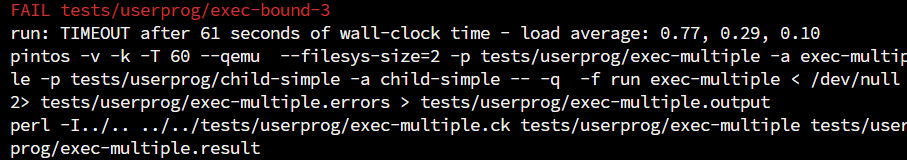
\includegraphics[width=\linewidth]{figures/exbound3.png}
    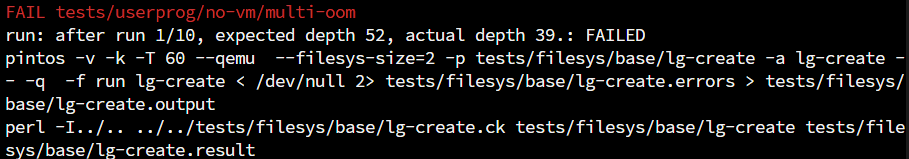
\includegraphics[width=\linewidth]{figures/muti.png}
\end{figure}
Their fixes are \textbf{validate\_user\_string ()} and \textbf{timely release memory} to prevent memory leaks.
\end{frame}

\begin{frame}[fragile]{results}
\begin{figure}
    \centering
    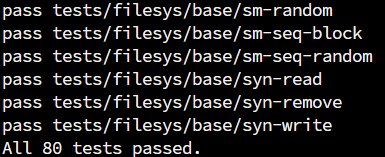
\includegraphics[width=\linewidth]{figures/result.png}
    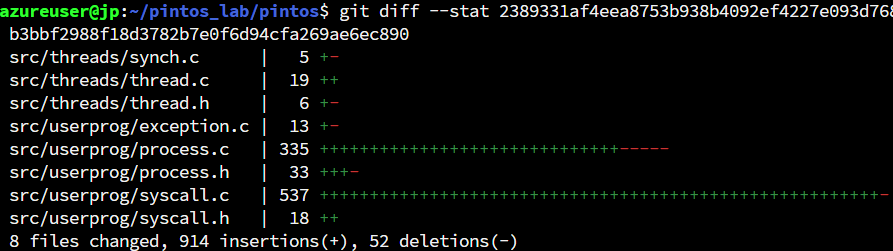
\includegraphics[width=\linewidth]{figures/git.png}
\end{figure}
\end{frame}

\begin{frame}[standout]
  \Large Thank you!\\
  Questions?
\end{frame}
\end{document}